\documentclass{article}
\usepackage{graphicx}
\usepackage{amssymb}
\usepackage{amsmath}
\usepackage{float}

\usepackage[margin=1in]{geometry}


\begin{document}



\title{16-720 Computer Vision: Homework 4}
\author{Xiang Zhi Tan}

\maketitle
\subsection*{Q1.1}
As learned in class, one of the property of the Fundamental Matrix is $p^TFp = 0$. When substituting p with the normalized points, we will get.
\begin{equation*}
\begin{pmatrix}
0 & 0 & 1
\end{pmatrix}
\begin{pmatrix}
F_{11}&F_{12}&F_{13}\\
F_{21}&F_{22}&F_{23}\\
F_{31}&F_{32}&F_{33}\\
\end{pmatrix}
\begin{pmatrix}
0\\
0\\
1\\
\end{pmatrix}
= 0
\end{equation*}
If we multiple the first point and the matrix, we will get
\begin{equation*}
\begin{pmatrix}
F_{31}&F_{32}&F_{33}\\
\end{pmatrix}
\begin{pmatrix}
0\\
0\\
1\\
\end{pmatrix}
= 0
\end{equation*}
If we multiple the two vectors we will get, $F_{33} \times 1 = 0$. That means that $F_{33}$ has to be equal to zero.
\subsection*{Q1.2}
First we used the property of $E = [t]_{\times} R$ and the fact that we are moving parallel to the x-axis to get the Essential Matrix.
\begin{equation*}
\begin{aligned}
E &= [t]_{\times} R\\
&=
\begin{pmatrix}
0& 0 & 0\\
0& 0 & -t_x\\
0& t_x & 0\\
\end{pmatrix} I\\
&=
\begin{pmatrix}
0& 0 & 0\\
0& 0 & -t_x\\
0& t_x & 0\\
\end{pmatrix}
\end{aligned}
\end{equation*}
To simply the problem, we assume that the intrinsic matrix, $K$ are the same for both cameras and their principal point to be the center of the image(both zeros). Now, we will try getting the fundemental matrix using $F = K^{-T}EK^{-1}$
\begin{equation*}
\begin{aligned}
F &= K^{-T}EK^{-1}\\
&=
\begin{pmatrix}
\frac{1}{f_x} &0 &0\\
0 & \frac{1}{f_y}&0\\
0 & 0 &1\\
\end{pmatrix}
\begin{pmatrix}
0& 0 & 0\\
0& 0 & -t_x\\
0& t_x & 0\\
\end{pmatrix}
\begin{pmatrix}
\frac{1}{f_x} &0 &0\\
0 & \frac{1}{f_y}&0\\
0 & 0 & 1\\
\end{pmatrix}\\
&=
\begin{pmatrix}
0& 0 & 0\\
0& 0 & \frac{-t_x}{f_y}\\
0& \frac{t_x}{f_y} & 0\\
\end{pmatrix}
\end{aligned}
\end{equation*}
The equation to generate an epipolar line is $l = Fx$. By applying the equation to 2 corresponding points on the images

\begin{equation*}
\begin{aligned}
l' &=
\begin{pmatrix}
0& 0 & 0\\
0& 0 & \frac{-t_x}{f_y}\\
0& \frac{t_x}{f_y} & 0\\
\end{pmatrix}
\begin{pmatrix}
x'\\
y'\\
1'\\
\end{pmatrix}
=
\begin{pmatrix}
0&
\frac{-t_x}{f_y}&
\frac{t_x y'}{f_y}\\
\end{pmatrix}\\
l &=
\begin{pmatrix}
0& 0 & 0\\
0& 0 & \frac{-t_x}{f_y}\\
0& \frac{t_x}{f_y} & 0\\
\end{pmatrix}
=
\begin{pmatrix}
0&
\frac{-t_x}{f_y}&
\frac{t_x y}{f_y}\\
\end{pmatrix}\\
\end{aligned}
\end{equation*}
As shown in the equality above the only difference between the two equations are that the constant(the last term) is different. The first two terms remain the same, means the slope of those two lines are the same. This means they are parallel.
\subsection*{Q1.3}
\begin{figure}[H]
    \centering
    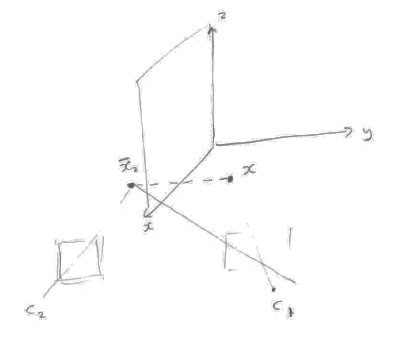
\includegraphics[width=6.5in]{./figures/q1_3}
\end{figure}

First we set the camera one to be the origin of the coordinates for the camera, this means it's camera matrix is $K[I|0]$. Through the image, we see that the camera 2's rotation matrix is actually a reflection on the mirror plane at $y=0$. This means that the difference between the cameras has to be a translation on the y-axis. Using a similar format as the previous questions, we can see construct the essential matrix as
\begin{equation*}
\begin{aligned}
E &= [t]_{\times} Reflection\\
&=
\begin{pmatrix}
0& 0 & t_y\\
0& 0 & 0\\
-t_y& 0 & 0\\
\end{pmatrix}
\begin{pmatrix}
1& 0 & 0\\
0& -1 & 0\\
0& 0 & 1\\
\end{pmatrix}
\\
&=
\begin{pmatrix}
0& 0 & t_y\\
0& 0 & 0\\
-t_y& 0 & 0\\
\end{pmatrix}
\end{aligned}
\end{equation*}
Now, we calculate the fundamental matrix, which gives us.
\begin{equation*}
\begin{aligned}
F &= K^{-T}EK^{-1}\\
&=
\begin{pmatrix}
\frac{1}{f_x} &0 &0\\
0 & \frac{1}{f_y}&0\\
0 & 0 &1\\
\end{pmatrix}
\begin{pmatrix}
0& 0 & t_y\\
0& 0 & 0\\
-t_y& 0 & 0\\
\end{pmatrix}
\begin{pmatrix}
\frac{1}{f_x} &0 &0\\
0 & \frac{1}{f_y}&0\\
0 & 0 & 1\\
\end{pmatrix}\\
&=
\begin{pmatrix}
0& 0 & \frac{t_y}{f_x}\\
0& 0 & 0\\
\frac{-t_y}{f_x}& 0 & 0\\
\end{pmatrix}
\end{aligned}
\end{equation*}
We need to show that $F$ is a skew-symmetric matrix. This means that $F = -F^T$
\begin{equation*}
\begin{aligned}
-F^T &=
-
\begin{pmatrix}
0& 0 & \frac{t_y}{f_x}\\
0& 0 & 0\\
\frac{-t_y}{f_x}& 0 & 0\\
\end{pmatrix}^T\\
&= 
-
\begin{pmatrix}
0& 0 & \frac{-t_y}{f_x}\\
0& 0 & 0\\
\frac{t_y}{f_x}& 0 & 0\\
\end{pmatrix}\\
&=
\begin{pmatrix}
0& 0 & \frac{t_y}{f_x}\\
0& 0 & 0\\
\frac{-t_y}{f_x}& 0 & 0\\
\end{pmatrix} = F\\
\end{aligned}
\end{equation*}
This proves that $F$ is a skew-symmetric matrix.
\subsection*{2.1}
The F matrix is as following
\begin{equation*}
F = 
\begin{pmatrix}
    0.0000   -0.0000    0.0031\\
   -0.0000   -0.0000    0.0000\\
   -0.0030    0.0000   -0.0121\\
\end{pmatrix}
\end{equation*}
Following is example of \textbf{displayEpipolarF} using the Eight point algorithm.
\begin{figure}[H]
    \centering
    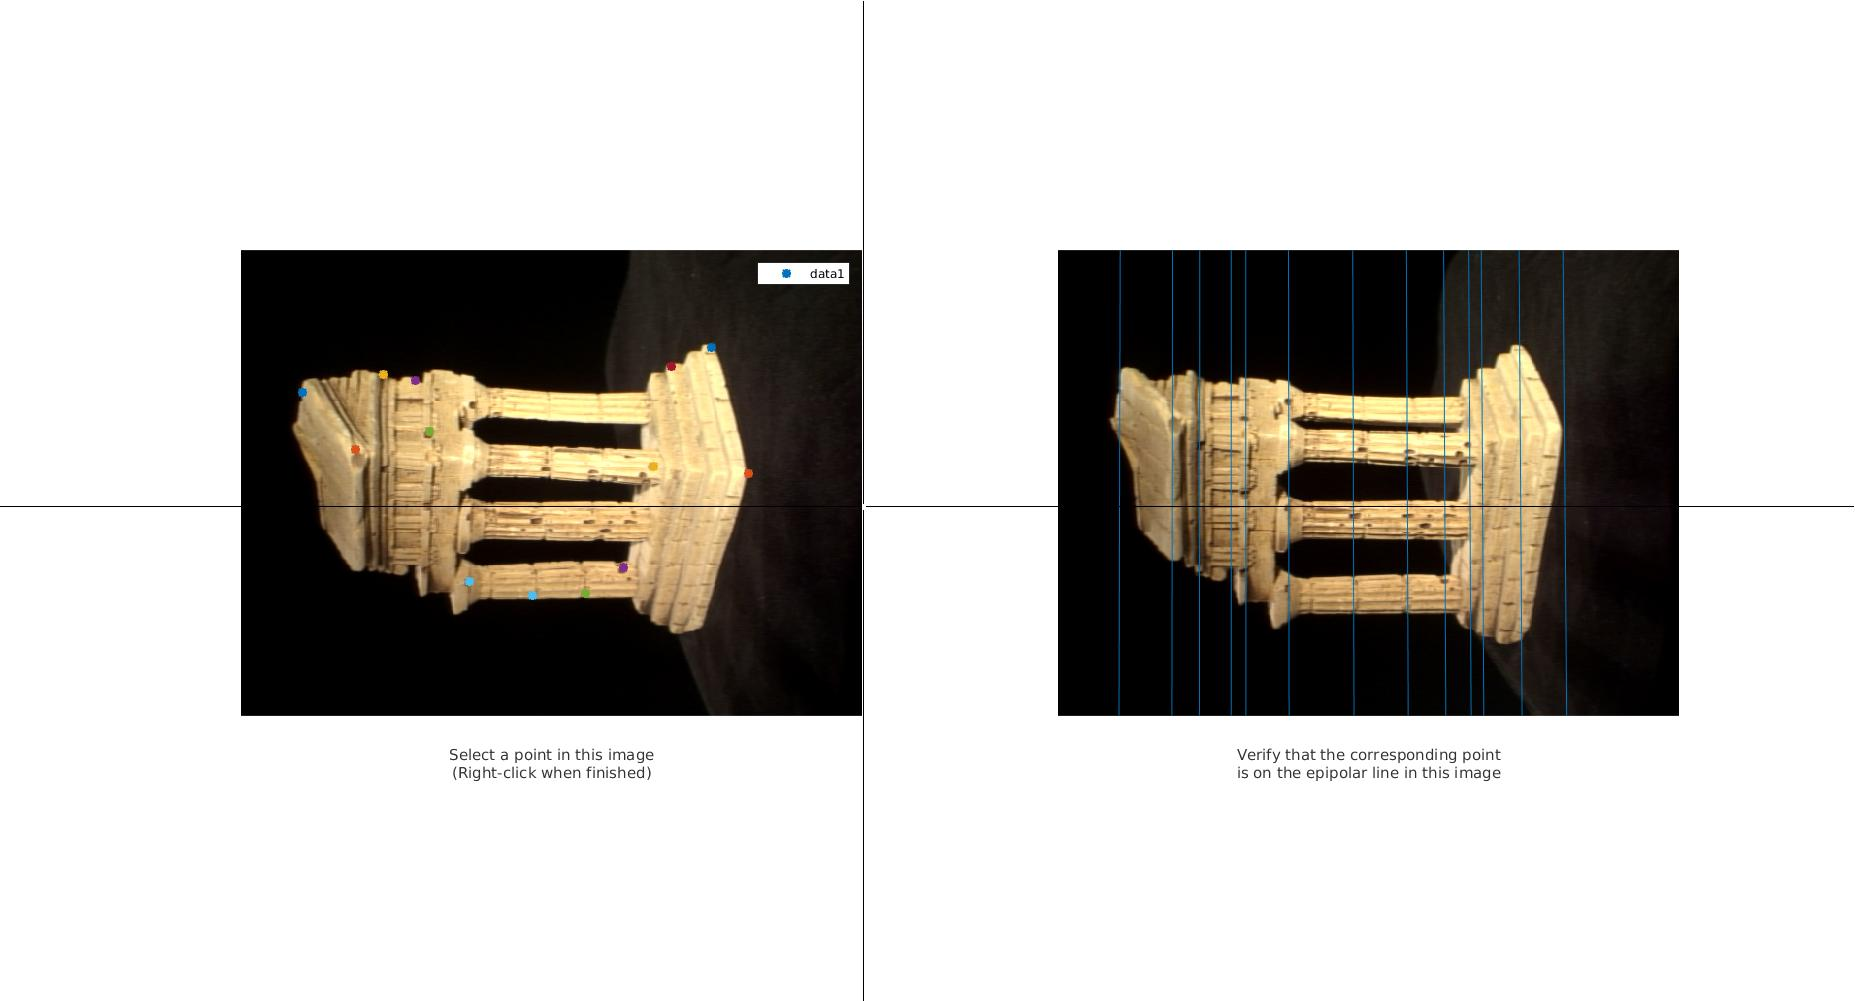
\includegraphics[width=6.5in]{./figures/q2_1}
\end{figure}
\subsection*{2.2}
Through selecting the picks [49 12 104 1 83 86 91], we get the following F matrix 
\begin{equation*}
F = 
\begin{pmatrix}
    0.0000 & -0.0000  &  0.0017\\
    0.0000 & -0.0000  & -0.0001\\
   -0.0018 &  0.0001  &  0.0091\\
\end{pmatrix}
\end{equation*}
Following is example of \textbf{displayEpipolarF} using the Seven point algorithm.
\begin{figure}[H]
    \centering
    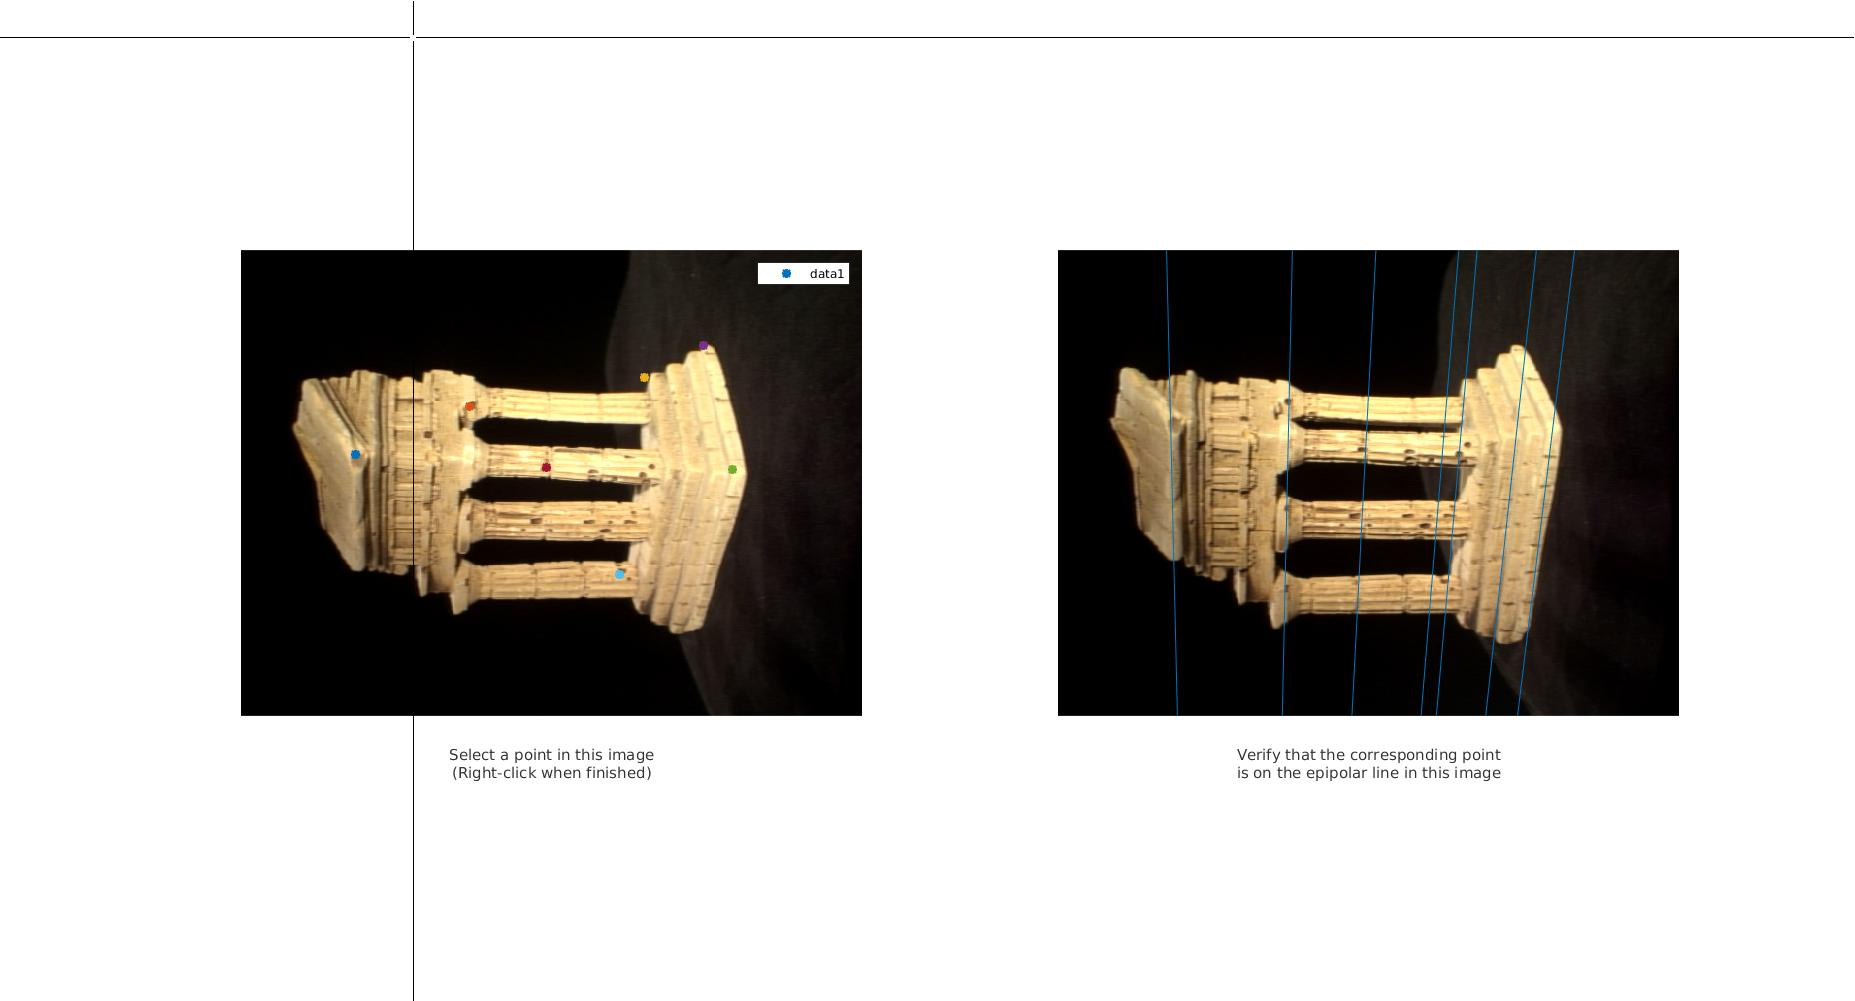
\includegraphics[width=6.5in]{./figures/q2_2}
\end{figure}

\subsection*{2.X}
My RANSAC method calculates the error by calculating $p'Fp$ for all the points. If the $F$ is perfect, $p'Fp$ should be $0$. I used this as the error matrix, where I consider pairs of points where $p'Fp < 0.005$ to be inliers. At each iteration, I save the index for the iteration where the inliers were the most. After 100 iterations, I recompute the F using the eightpoint algorithm with those saved inliers.\\
Following is the F generated by RANSAC:
\begin{equation*}
F = 
\begin{pmatrix}
    0.0000  &  0.0000&   -0.0023\\
    0.0000   &-0.0000&   -0.0000\\
    0.0022   &-0.0000&    0.0107\\
\end{pmatrix}
\end{equation*}
Following is example of \textbf{displayEpipolarF} using the F generated by RANSAC
\begin{figure}[H]
    \centering
    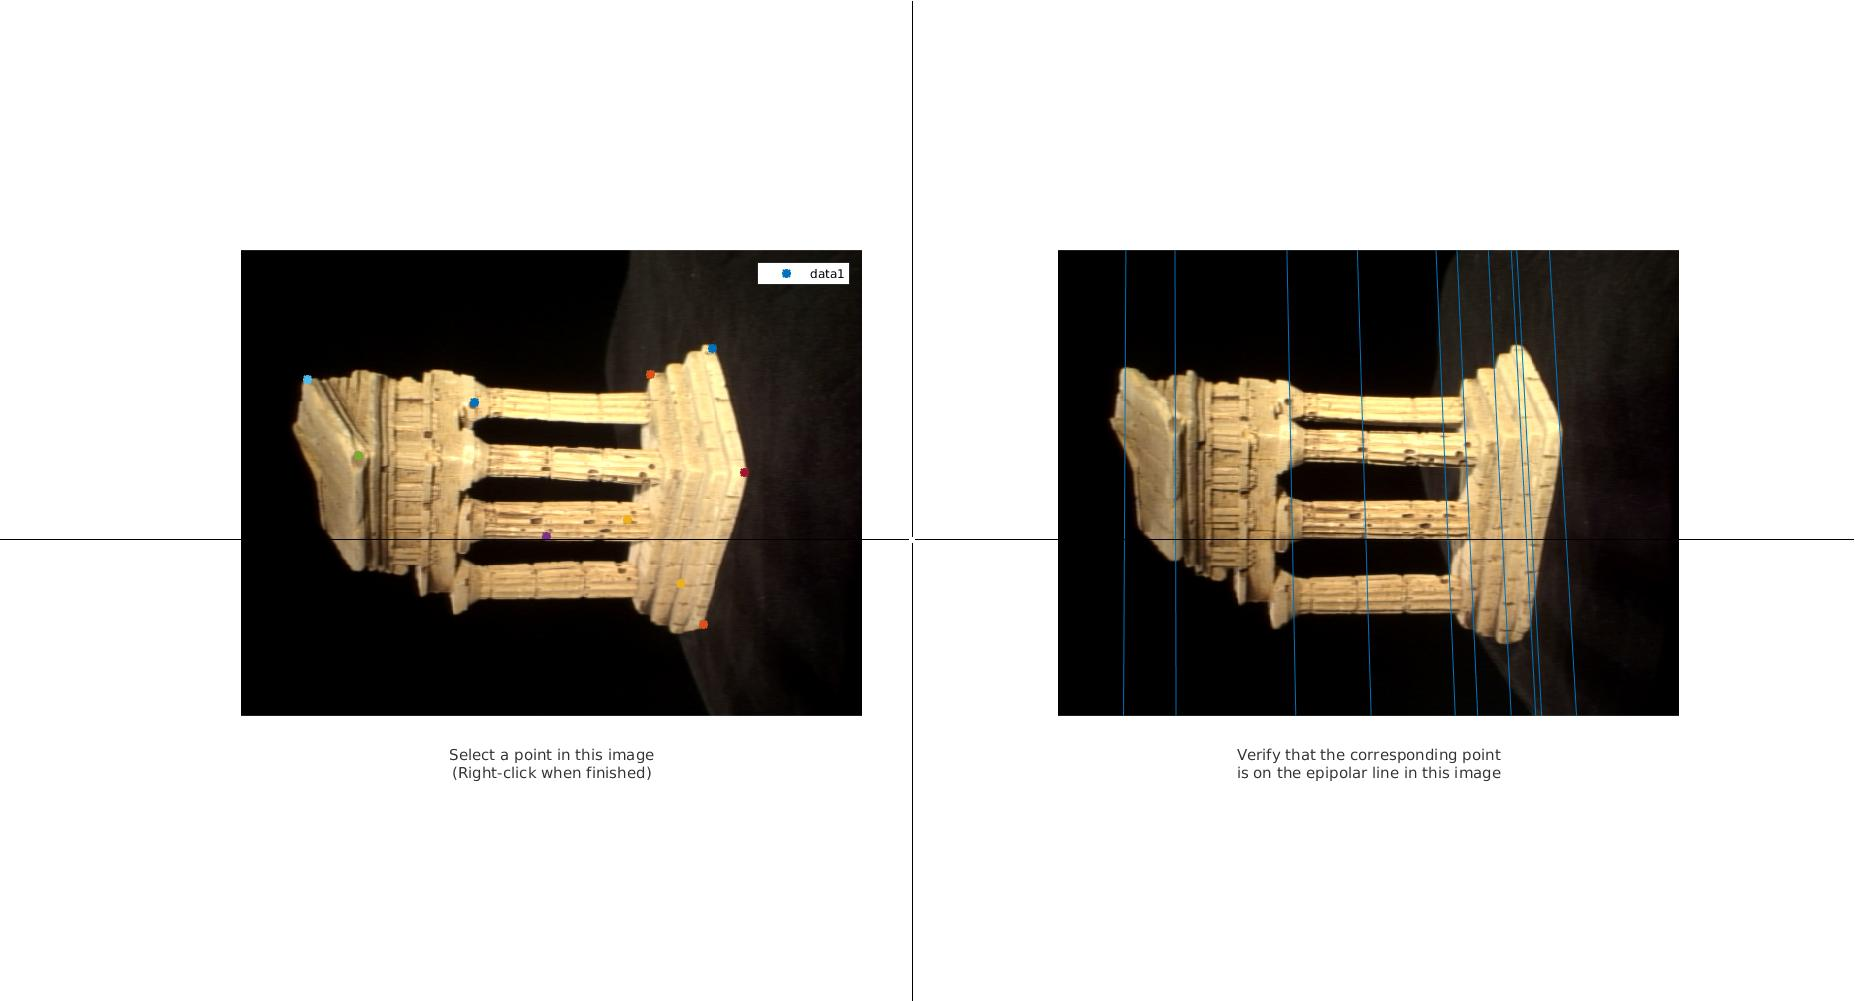
\includegraphics[width=6.5in]{./figures/randsac}
\end{figure}
If we did not use RANSAC, this will be the F generated by the eight point algorithm:
\begin{equation*}
F = 
\begin{pmatrix}
   -0.0000  &  0.0000&   -0.0008\\
   -0.0000  &  0.0000&    0.0011\\
    0.0012  & -0.0017&    0.0044\\
\end{pmatrix}
\end{equation*}
Following is example of \textbf{displayEpipolarF} without RANSAC
\begin{figure}[H]
    \centering
    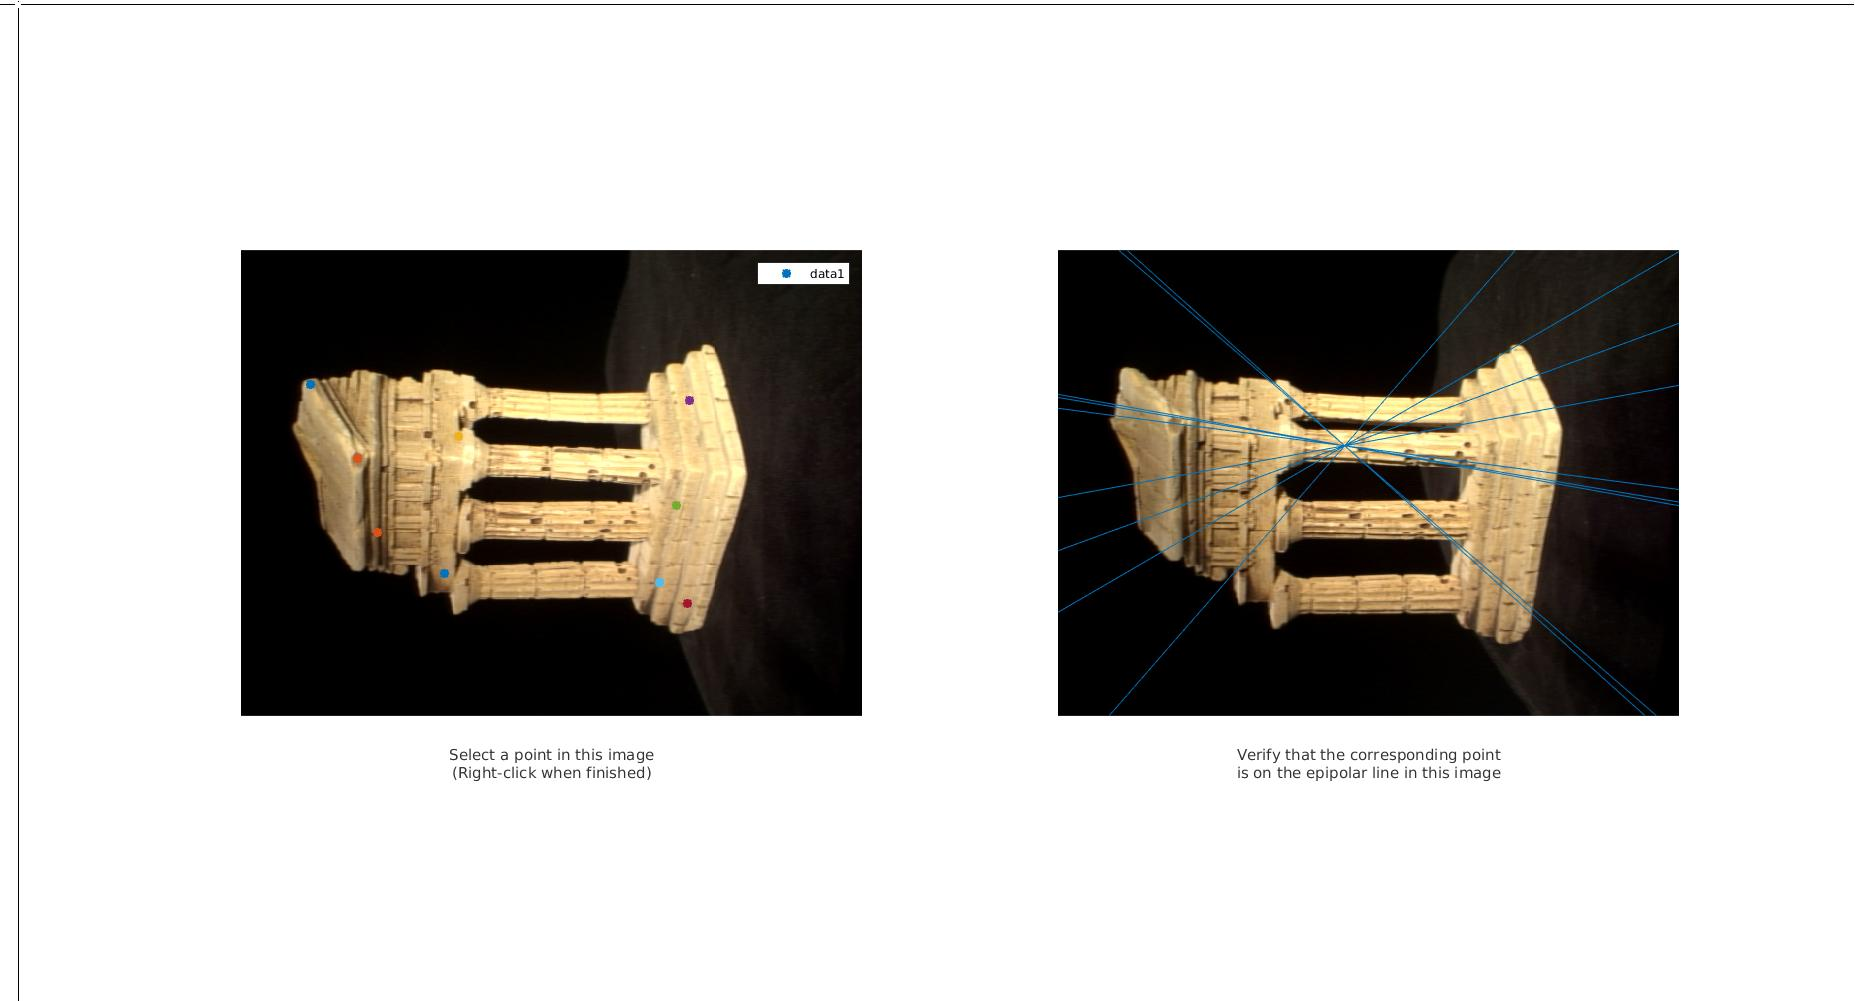
\includegraphics[width=6.5in]{./figures/no_randsac}
\end{figure}

\subsection*{2.3}
Following is the F matrix used for the estimation.
\begin{equation*}
F = 
\begin{pmatrix}
    0.0000  & -0.0000  &  0.0031 \\
   -0.0000  & -0.0000  &  0.0000 \\
   -0.0030  &  0.0000  & -0.0121 \\
\end{pmatrix}
\end{equation*}
Following is the Essential matrix estimated from F, K1 and K2.
\begin{equation*}
E = 
\begin{pmatrix}
    0.0568   &-1.1031  & 4.5982\\
   -0.1539  & -0.0020  & -0.0121\\
   -4.6073  & -0.1472  & -0.0014\\
\end{pmatrix}
\end{equation*}
\subsection*{2.4}
For triangulation, I used the Linear triangulation method which calculates the triangulation based on the difference in points. Using that method, I found my reprojection error is $6.2508 \times 10^4$ 
\subsection*{2.6}
Following is a screenshot of \textbf{epipolarMatchGUI} with some detected correspondences.
\begin{figure}[H]
    \centering
    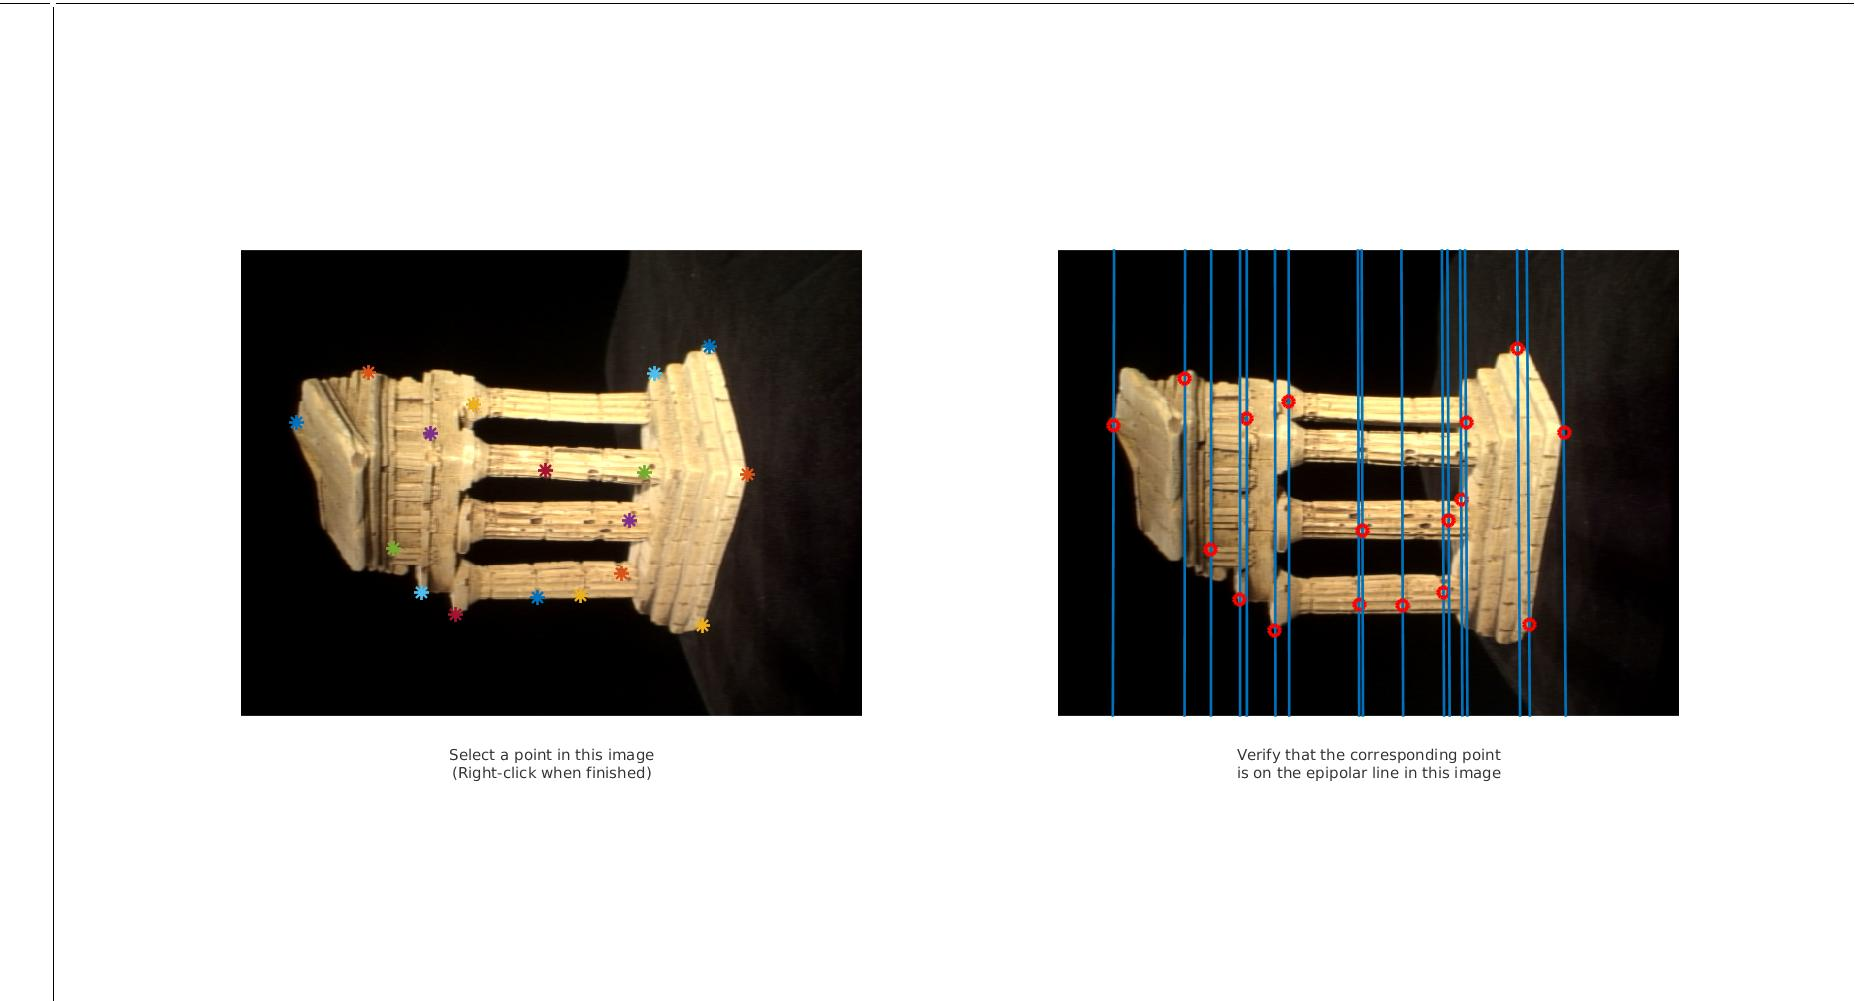
\includegraphics[width=6.5in]{./figures/q2_6}
\end{figure}
\subsection*{2.7}
Following are a few 3D visualization of 3D point cloud.
\begin{figure}[H]
    \centering
    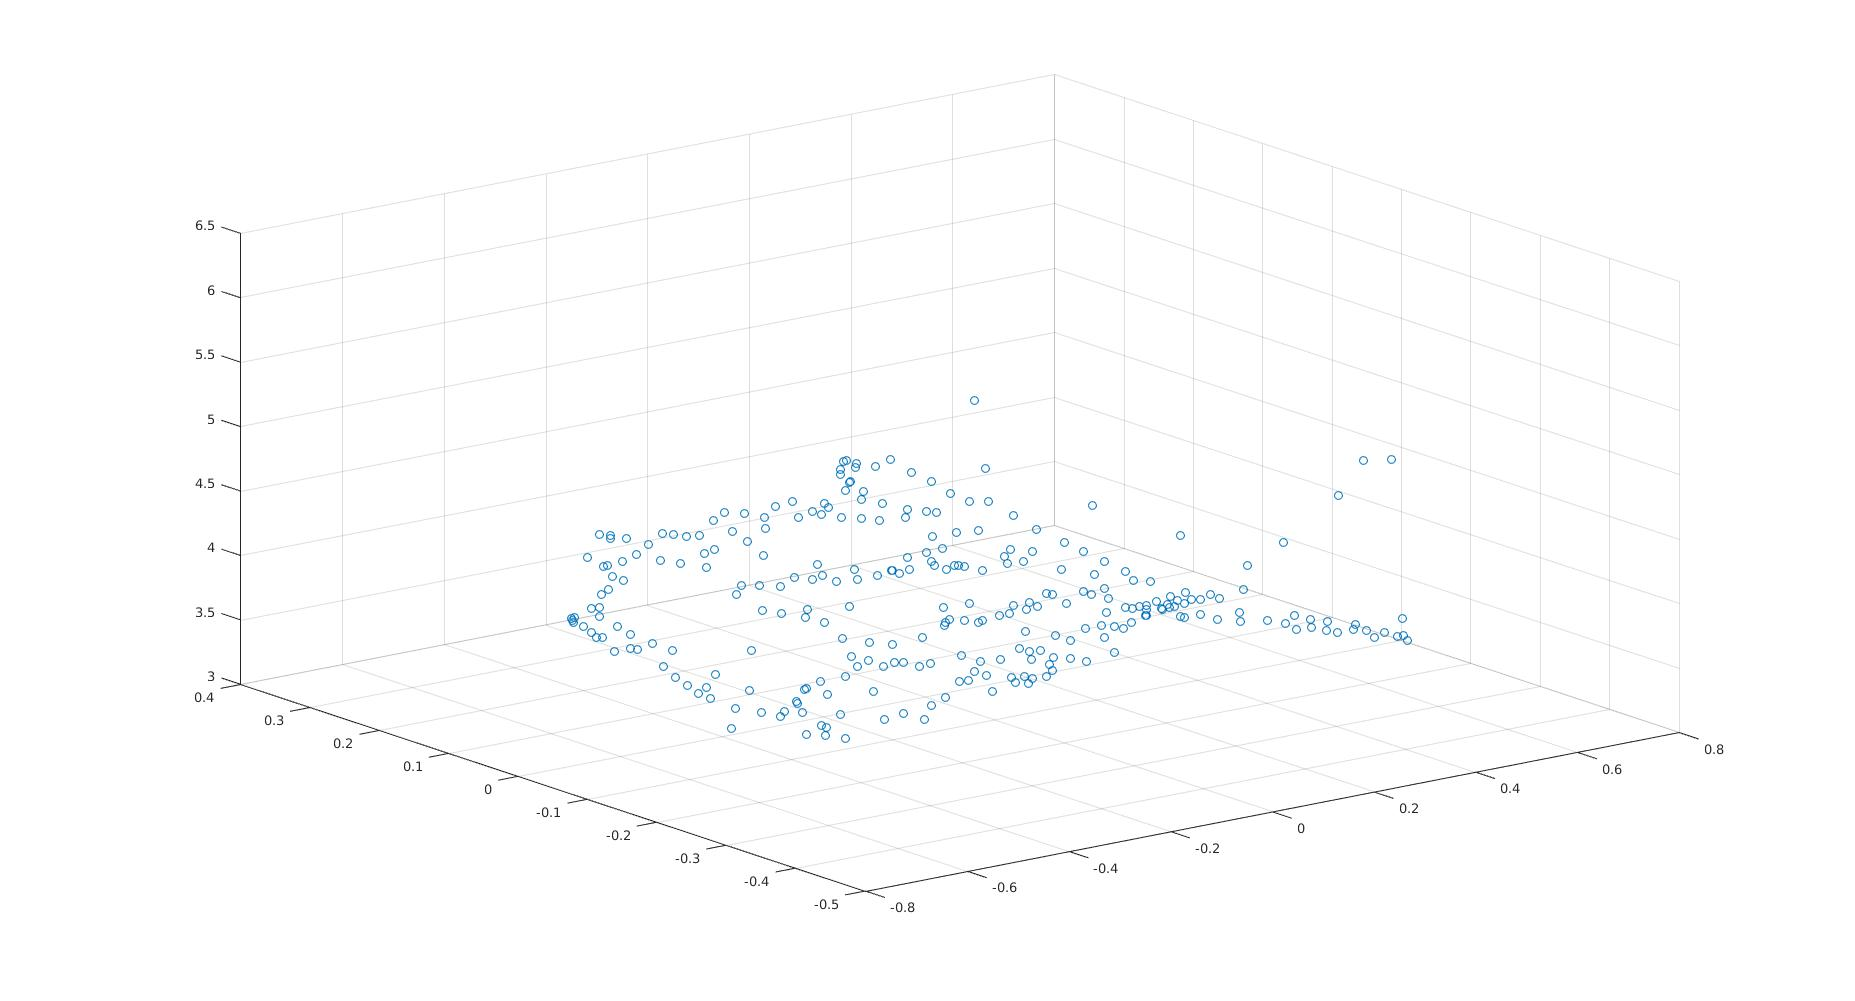
\includegraphics[width=6.5in]{./figures/q2_7_1}
\end{figure}
\begin{figure}[H]
    \centering
    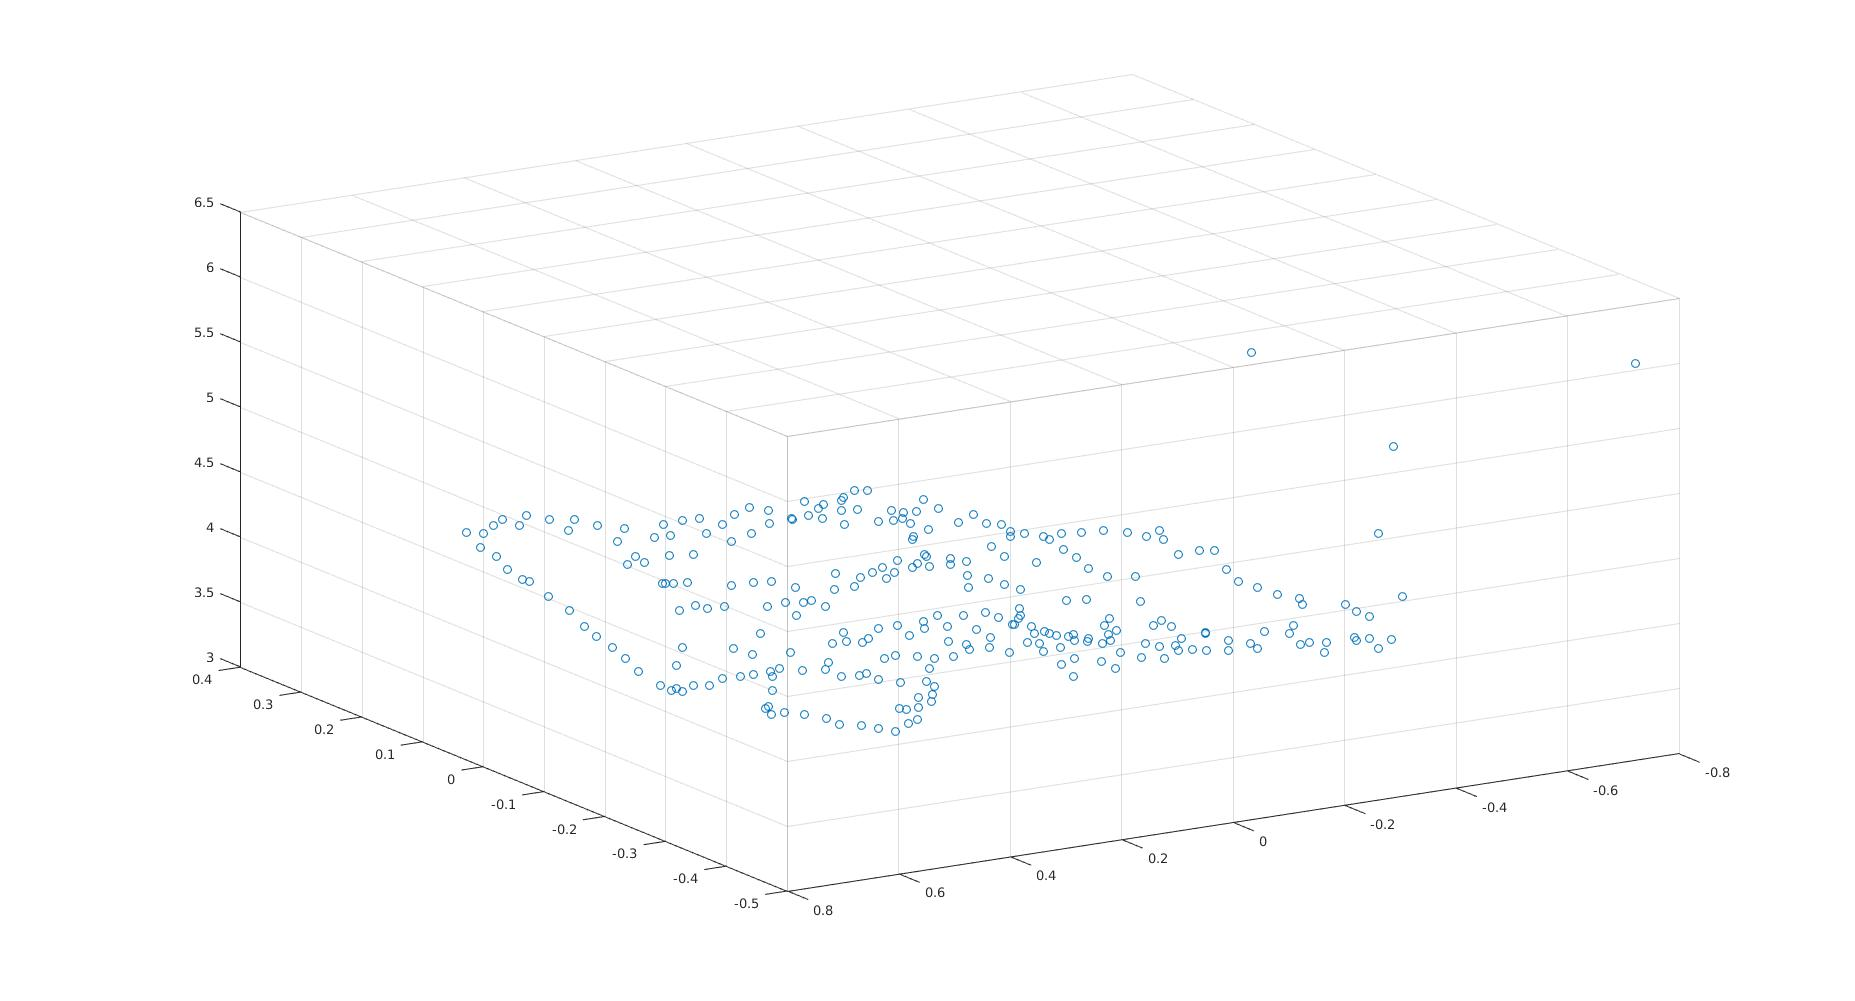
\includegraphics[width=6.5in]{./figures/q2_7_4}
\end{figure}
\begin{figure}[H]
    \centering
    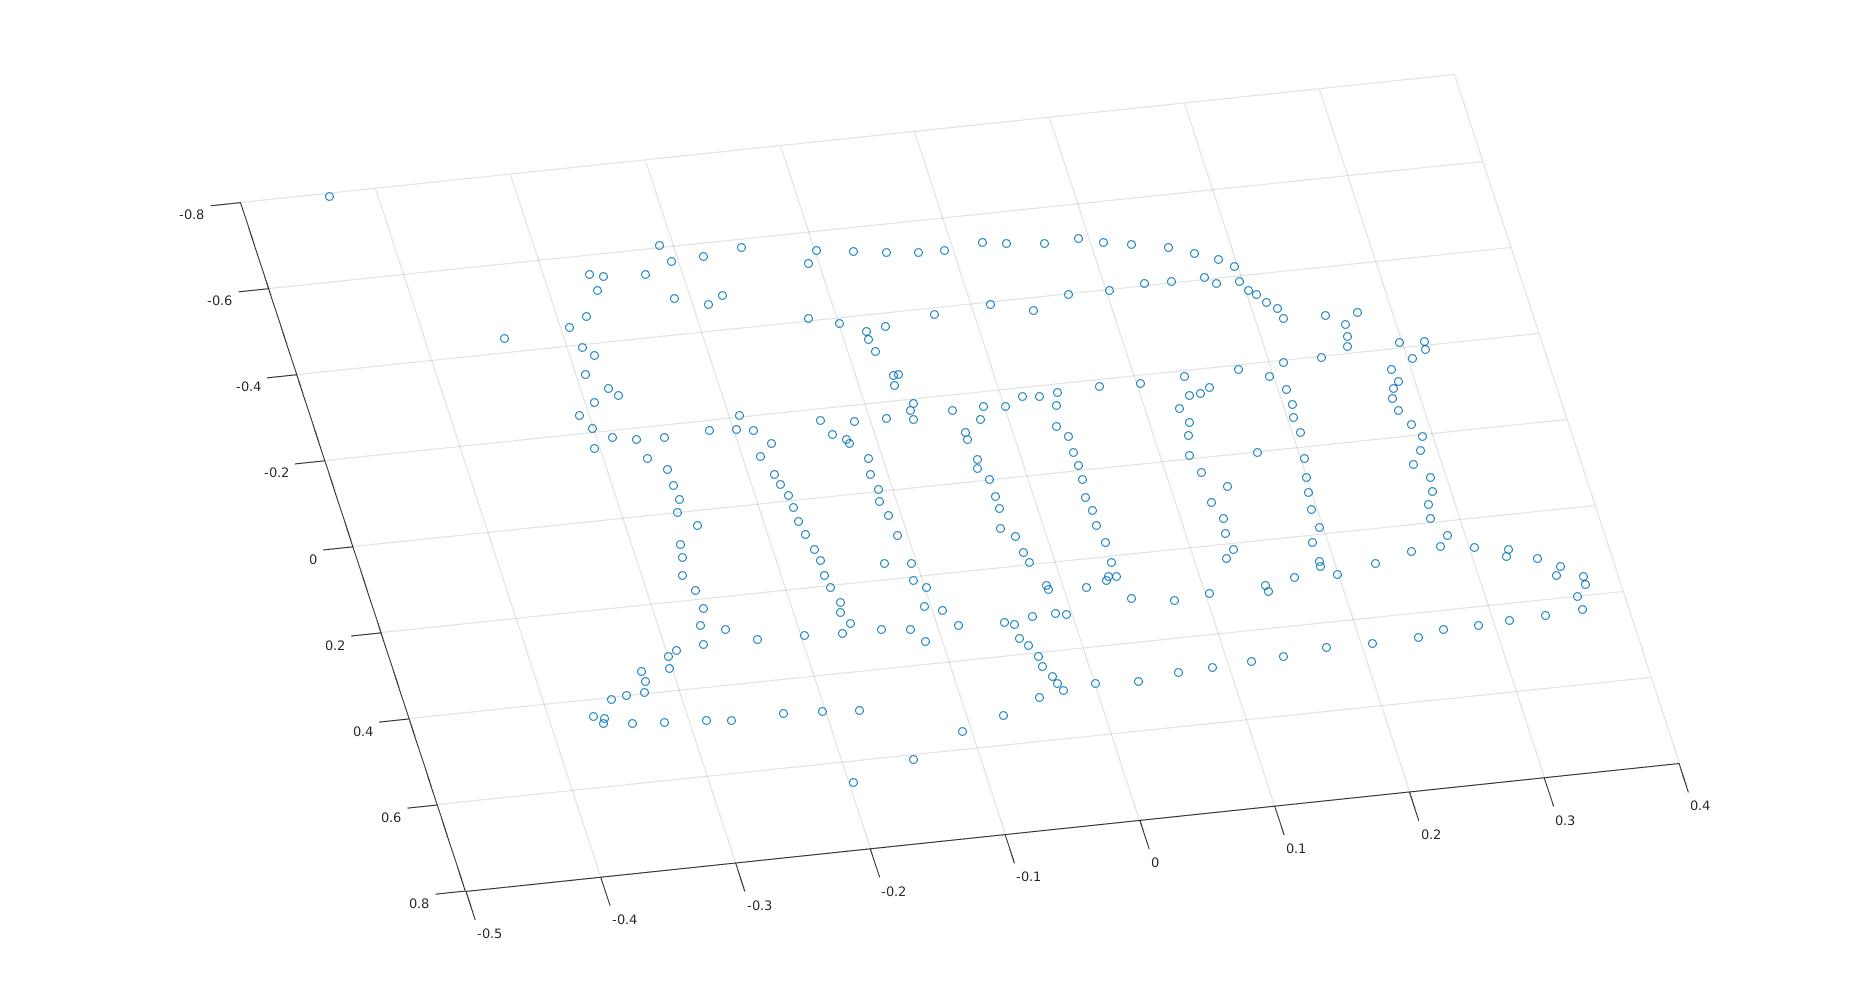
\includegraphics[width=6.5in]{./figures/q2_7_2}
\end{figure}
\begin{figure}[H]
    \centering
    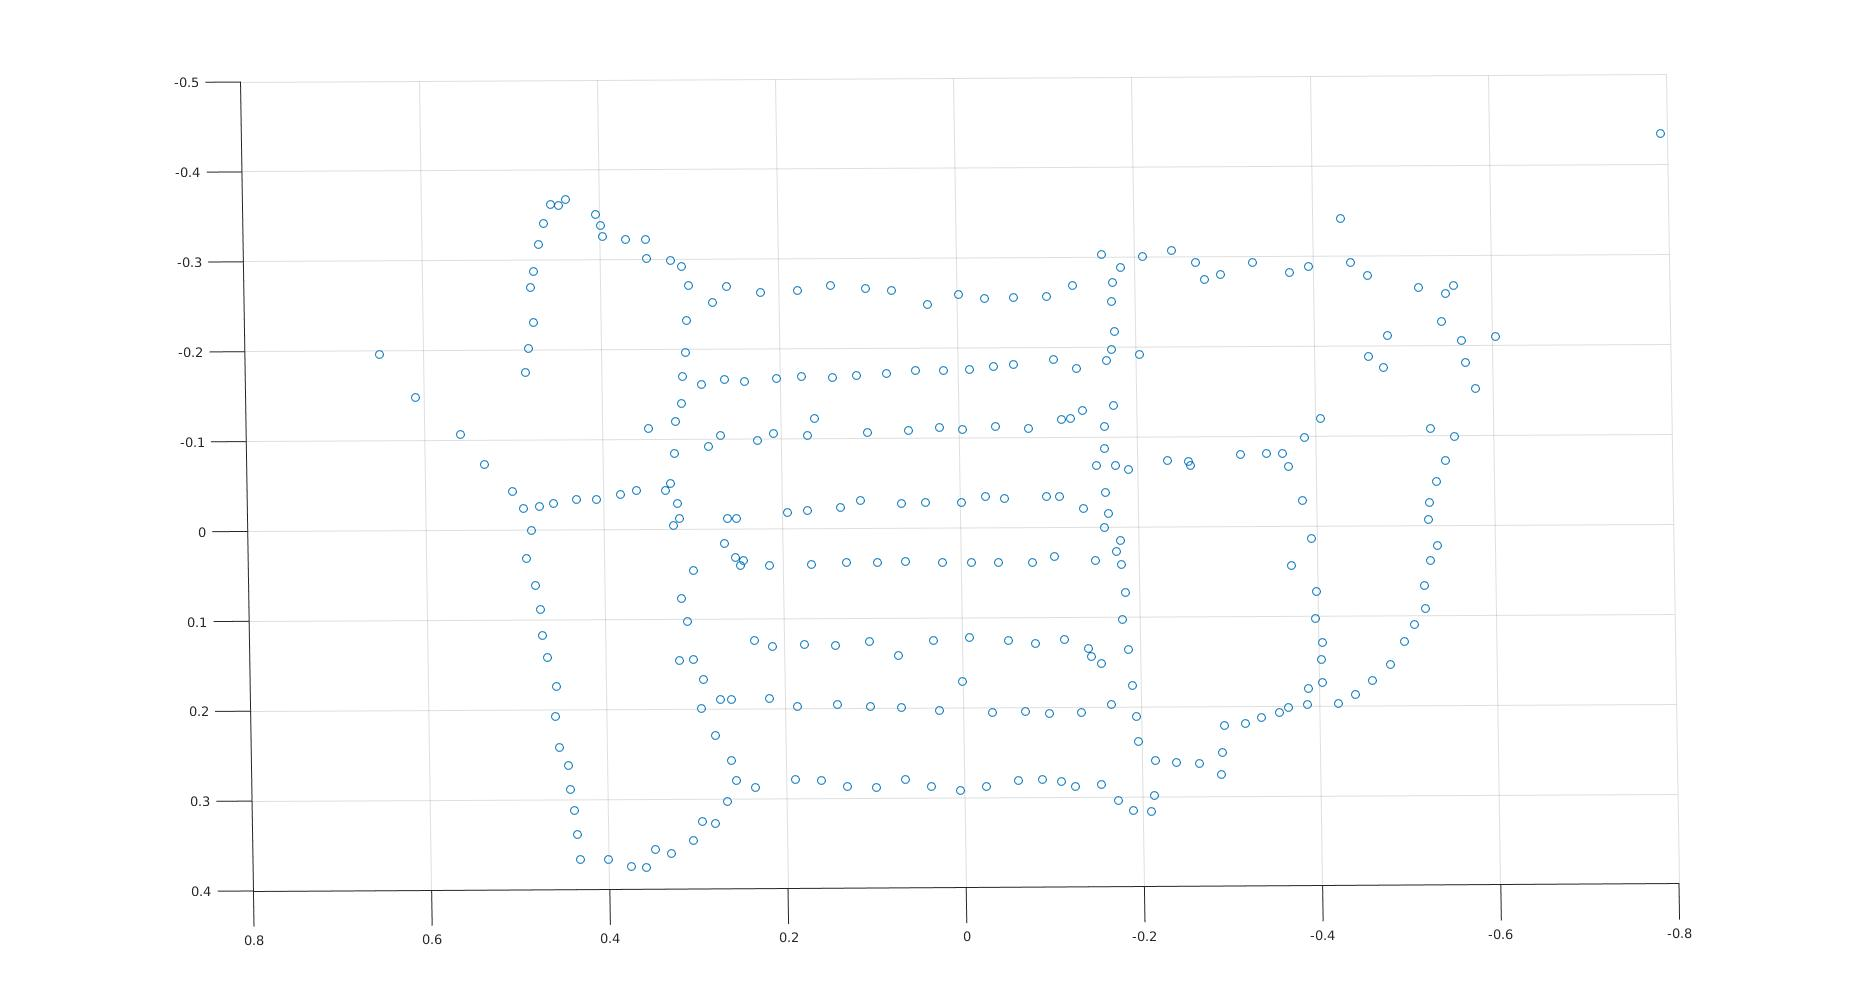
\includegraphics[width=6.5in]{./figures/q2_7_3}
\end{figure}
\end{document}